\documentclass{beamer}
\mode<presentation>
\usepackage{amsmath}
\usepackage{amssymb}
%\usepackage{advdate}
\usepackage{adjustbox}
\usepackage{subcaption}
\usepackage{enumitem}
\usepackage{multicol}
\usepackage{mathtools}
\usepackage{listings}
\usepackage[english]{babel} % To obtain English text with the blindtext package
\usepackage{blindtext}
\usepackage{url}
\def\UrlBreaks{\do\/\do-}
\usetheme{Boadilla}
\usecolortheme{lily}
\setbeamertemplate{footline}
{
  \leavevmode%
  \hbox{%
  \begin{beamercolorbox}[wd=\paperwidth,ht=2.25ex,dp=1ex,right]{author in head/foot}%
    \insertframenumber{} / \inserttotalframenumber\hspace*{2ex} 
  \end{beamercolorbox}}%
  \vskip0pt%
}
\setbeamertemplate{navigation symbols}{}



\title{Evaluating Scalable Bayesian Deep Learning
Methods for Robust Computer Vision. \\ Fredrik K. Gustafsson, Martin Danelljan, Thomas B. Schon}
\author{ Abhishek Sabnis \\ ME18BTECH11049 \\IIT Hyderabad.}


\date{\today} 
\begin{document}

\begin{frame}
\titlepage
\end{frame}

\section*{Outline}
\begin{frame}
\tableofcontents
\end{frame}
\section{Introduction}

\begin{frame}
\frametitle{Introduction}
%
    \hspace{0.3cm} Although DL technique works, it’s most of the time unclear why deep learning works. The majority of these models fail to properly capture the uncertainty inherent in their predictions. Estimating this predictive uncertainty can be crucial, for example in automotive application. If the car is unsure where there is a pedestrian on the road, we would expect it to let the driver take charge. 
    
    \vspace{0.3cm}
    
    \hspace{0.3cm} While different scalable methods recently have emerged, no extensive comparison has been performed in a real-world setting. This paper proposes a comprehensive evaluation framework for scalable  uncertainty estimation methods in deep learning.
%

\end{frame}

%-------------------------------------------------------------------------------------

\section{Types of Uncertainty}
\begin{frame}
\frametitle{Types of Uncertainty}

There are two major different types of uncertainty in deep learning: epistemic uncertainty and aleatoric uncertainty. 

\vspace{0.3cm}

\begin{itemize}
  \item \textbf{Epistemic Uncertainty}: Accounts for uncertainty in the DNN
model parameters, due to limited training data

  \item \textbf{Aleatoric Uncertainty}: It is the uncertainty arising from the natural stochasticity of observations. Aleatoric uncertainty cannot be reduced even when more data is provided. 
\end{itemize}

\end{frame}



\begin{frame}
\frametitle{Types of Uncertainty}

\begin{itemize}
\item In many computer vision applications, this aleatoric uncertainty can be effectively estimated by letting a DNN directly output the conditional distribution $p(y|x)$ of the target given the input.
\item But this does not capture epistemic uncertainty, as information about the uncertainty in the model parameters is disregarded. This often leads to highly confident predictions that are incorrect, especially for inputs x that are not well-represented by the training distribution.
\end{itemize}


\end{frame}

%---------------------------------------------------------------------------------

\subsection{Estimating Aleatoric Uncertainty}
\begin{frame}
\frametitle{Estimating Aleatoric Uncertainty}

We now formulate equation to estimate Aleatoric Uncertainty of DNN model.

\vspace{0.3cm}

\hspace{0.3cm} In classification problems, aleatoric uncertainty is commonly captured by predicting a categorical distribution $p(y|x, θ)$. This is implemented by letting the DNN predict logit scores $f_\theta (x) \in R^C  $  , which are then normalized by a Softmax function.

\begin{align}
\begin{split}
 p(y|x, \theta) &= Cat(y; s_\theta (x)) ,
\\
 s_\theta (x) &= Softmax(f_\theta(x)) .
\end{split}
\end{align}

\end{frame}



\begin{frame}
\frametitle{Estimating Aleatoric Uncertainty}

\hspace{0.3cm} Given a training set of i.i.d. sample pairs $ D = \{X, Y\} = \{(x_i, y_i)\}_{i=1}^N , (x_i,y_i) \sim p(x,y)$, the data likelihood is obtained as $p(Y|X, \theta) = \prod_{i=1}^{N} p(y_i| x_i, \theta)$. 

\vspace{0.3cm}

\hspace{0.3cm} The MLE of the model parameters, $\theta^{^}_{MLE}$, is obtained by minimizing negative log likelihood $-\sum_i log p(y_i|x_i,\theta)$. For Categorical model this is equivalent to minimizing Cross entropy loss.

\end{frame}




\begin{frame}
\frametitle{Estimating Aleatoric Uncertainty}

\hspace{0.3cm} In regression, the most common approach is to let DNN directly predict targets, $y^* = f_{\theta^{^}} $ $(x^*)$. The parameters $\hat{\theta}$ is learned by minimizing $L^2$ loss. But this does not capture aleatoric uncertainty. Instead, we predict the distribution $p(y|x,\theta)$, similar to classification case. 

\begin{align}
\begin{split}
 p(y|x, \theta) &= N(y; \mu_\theta(x), \sigma_\theta^2 (x)) ,
\\
 f_\theta (x) &= [\mu_\theta(x), log \sigma_\theta^2 (x)] .
\end{split}
\end{align}

The model parameters are learnt by minimizing negative log likelihood $-\sum_i log p(y_i|x_i,\theta)$

\end{frame}

%---------------------------------------------------------------------

\subsection{Estimating Epistemic Uncertainty}
\begin{frame}
\frametitle{Estimating Epistemic Uncertainty}

While the above model captures the uncertainty in data, we are still yet to capture the uncertainty arising from model parameter $\theta$. The aim is to utilize the posterior distribution $p(\theta | D)$, which is obtained from data likelihood and a chosen prior $p(\theta)$ by applying Bayes Theorem. 

\begin{align}
\begin{split}
 p(y^*|x^*, D) &= \int p(y^*|x^*, \theta) p(\theta | D) d\theta ,
\\
  &= \frac{1}{M} \sum_{i=1}^{M} p(y^*| x^*, \theta^{(i)}), \theta^{(i)} \sim p(\theta | D) .
\end{split}
\end{align}

where $(x^*, y^*)$ is test data set and D is the given training data.

\end{frame}





\begin{frame}
\frametitle{Estimating Epistemic Uncertainty}

\hspace{0.3cm} For the Categorical model, $\hat{p}(y^* | x^*, D) = Cat(y^*; \hat{s}(x^*))$, where $\hat{s}(x^*) = \frac{1}{M} \sum_{i=1}^{M} s_{\theta^{(i)}} (x^*)$ and $s_{\theta^{(i)}} (x^*)$ is the softmax of logits function.
\vspace{0.3cm}

\hspace{0.3cm} For the Regression model, we use uniformly weighted mixture of Gaussian model to calculate $\hat{p}(y^* | x^*, D)$. We approximate this mixture with a single Gaussian as follows - 

\end{frame}







\begin{frame}
\frametitle{Estimating Epistemic Uncertainty}

\begin{align}
\begin{split}
 p(y^*|x^*, D) &= \frac{1}{M} \sum_{i=1}^{M} p(y^*| x^*, \theta^{(i)})
\\
  &= \frac{1}{M} \sum_{i=1}^{M} N(y^*; \mu_{\theta^{(i)}} (x^*), \sigma_{\theta^{(i)}}^2 (x^*)) 
\\
  &= N(y^*; \hat{\mu}(x^*), \hat{\sigma}^2 (x^*))
\end{split}
\end{align}

where
$\hat{\mu}(x) = \frac{1}{M} \sum_{i=1}^{M} \mu_{\theta^{(i)}} (x) $, 

\vspace{0.3cm}

$\hat{\sigma}^2 (x) = \frac{1}{M} \sum_{i=1}^{M} ((\mu_{\theta^{(i)}} (x) -  \hat{\mu}(x) )^2 + \sigma_{\theta^{(i)}}^2 (x)) )$

\end{frame}



%-------------------------------------------------------------------
\section{Popular Framework}
\begin{frame}
\frametitle{Popular Framework}

\hspace{0.3cm} Among scalable methods of Bayesian inference, MC dropout and Ensembling are the widely employed methods.

\vspace{0.3cm}

\hspace{0.3cm} While scalable techniques for epistemic uncertainty estimation recently have emerged, the research community however lacks a common and comprehensive evaluation framework for such methods.

\vspace{0.3cm}

\hspace{0.3cm}The paper propose an evaluation framework that actually enables a conclusive ranking of the compared methods.


\end{frame}
%-----------------------------------------------------------------

\subsection{MC Dropout}
\begin{frame}
\frametitle{MC Dropout}

\hspace{0.3cm} Modeling uncertainty with Monte Carlo dropout works by running multiple forward passes trough the model with a different dropout masks every time.To derive the uncertainty for one sample x, we collect the predictions of T inferences with different dropout masks.

\vspace{0.3cm}

\hspace{0.3cm} By computing the average and the variance of this sample we get an ensemble prediction, which is the mean of the models posterior distribution for this sample and an estimate of the uncertainty of the model regarding x.

\end{frame}
%---------------------------------------------------------------------------------

\subsection{Ensembling}
\begin{frame}
\frametitle{Ensembling}

We create a parametric model $p(y|x,\theta)$ of the conditional distribution using a DNN, and learn multiple point estimates $\hat{\theta}^{(m)}$ by repeatedly minimizing MLE with random initialization. We then average over the parametric models to obtain the following predictie distribution - 

\begin{equation}
    \hat{p} (y^*|x^*) = \frac{1}{M} \sum_{m=1}^{M} p(y^* | x^*, \theta^{m})
\end{equation}

\end{frame}
%-------------------------------------------------------------------------------------


\section{Evaluation Metrics}
\subsection{AUSE}
\begin{frame}
\frametitle{Evaluation Metrics}

\textbf{Area Under the Sparsification Error curve (AUSE)}

\vspace{0.3cm}

We evaluate the methods in terms of the Area Under the Sparsification Error curve (AUSE) metric. The metric reveals how well the estimated uncertainty can be used to sort predictions from worst (large true prediction error) to best (small prediction error). We compute AUSE in terms of Root Mean Squared Error (RMSE) and based on all pixels in the entire evaluation dataset.

\end{frame}




\subsection{AUCE}
\begin{frame}
\frametitle{Evaluation Metrics}

\textbf{Area Under the Calibration Error curve (AUCE)}

\vspace{0.3cm}

\hspace{0.3cm} Since our models output the mean $\mu$ and variance $\sigma^2$ of a Gaussian distribution for each pixel, we can construct pixel-wise prediction intervals $\mu \pm \Phi^{-1} (\frac{p+1}{2}) \sigma$ of confidence level $p \in [0,1]$, where $\Phi$ is the CDF of the standard normal distribution. 

\vspace{0.3cm}

\hspace{0.3cm} When computing the proportion of pixels for which the prediction interval covers the true target $y \in R$, we expect this value, denoted by $\hat{p}$, to equal $p \in [0,1]$ for a perfectly calibrated model. 

\vspace{0.3cm}

\hspace{0.3cm} We compute the absolute error with respect to perfect calibration, $|p - \hat{p} |$, for 100 values of $p \in [0,1]$ and use the area under this curve as our metric, which we call Area Under the Calibration Error curve (AUCE).


\end{frame}
%------------------------------------------------------------------------------

\section{Experiments}
\subsection{Depth Completion}
\begin{frame}
\frametitle{Depth Completion}

\hspace{0.3cm} In depth completion, we are given an image $x_{img} \in R^{h\times w\times 3}$ from a forward-facing camera and an associated sparse depth map $x_{sparse} \in R^{h\times w}$

\vspace{0.3cm}

\hspace{0.3cm} DNN model based on Resnet 34 architecture is used. Gaussian model (2) is employed in the final layer, outputting both $\mu$ and $log \sigma^2$. We now train the model using both MC dropout and Ensembling techniques.

\end{frame}



\begin{frame}{Depth Completion}

\begin{figure}
\centering
    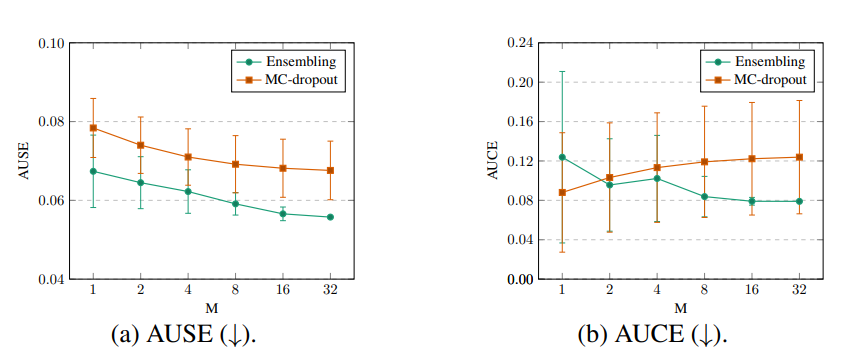
\includegraphics[width=10cm]{depth.png}
    \caption{The plots show a comparison of ensembling and MC-dropout in terms of
AUSE, AUCE on the depth completion validation dataset, for different number of samples M}
    \label{fig:question}
\end{figure}

\end{frame}

%-------------------------------------------------------------------------------------

\subsection{Street-Scene Semantic Segmentation}
\begin{frame}
\frametitle{Street-Scene Semantic Segmentation}

\hspace{0.3cm} We are given an image $x_{img} \in R^{h\times w\times 3}$ from a forward-facing camera The goal is to predict y of size h $\times$ w, in which each pixel is assigned to one of C different class label.

\vspace{0.3cm}

The input image x is processed by a ResNet101. The feature maps is further processed and upsampled using bilinear interpolation. The conventional Categorical model (1) is used for each pixel. Finally trained using MC Dropout and Ensembling techniques.

\end{frame}



\begin{frame}{Street-Scene Semantic Segmentation}

\begin{figure}
\centering
    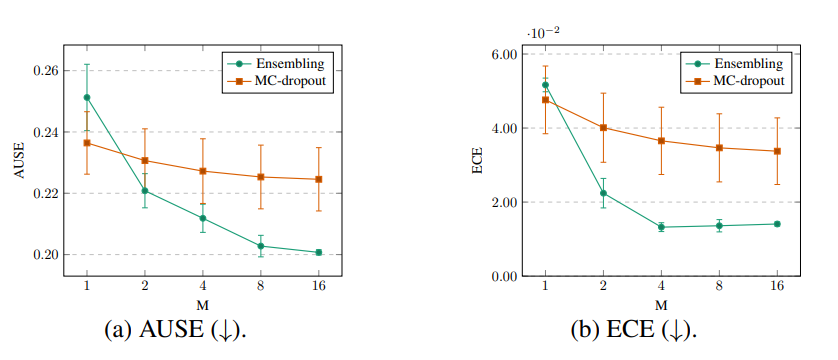
\includegraphics[width=10cm]{seg.png}
    \caption{The plots show a comparison of ensembling and MC-dropout in terms of AUSE, AUCE on the Street-scene semantic segmentation validation dataset, for different number of samples M}
    \label{fig:question}
\end{figure}

\end{frame}
%-------------------------------------------------------------------------------

\section{Conclusion}

\begin{frame}
\frametitle{Conclusion}

\hspace{0.3cm} Provided the first properly extensive and conclusive comparison of ensembling and MC-dropout, the results of which demonstrates that ensembling consistently provides more reliable and practically useful uncertainty estimates.

\vspace{0.3cm} 

\hspace{0.3cm} We observe that the metrics clearly improve as functions of M for both ensembling and MC-dropout, demonstrating the importance of epistemic uncertainty estimation.

\vspace{0.3cm} 

\hspace{0.3cm} MC-dropout has a large design-space compared to ensembling. But the success of ensembling is due to the random initialization, to capture the important aspect of multi-modality present in the posterior distribution.

\end{frame}



\begin{frame}
\frametitle{References}

Evaluating Scalable Bayesian Deep Learning
Methods for Robust Computer Vision. Fredrik K. Gustafsson, Martin Danelljan, Thomas B. Schon¨


Department of Information Technology, Uppsala University, Sweden Computer Vision Lab, ETH Zurich, Switzerland

\end{frame}



\end{document}
